%%%%%%%% ICML 2021 EXAMPLE LATEX SUBMISSION FILE %%%%%%%%%%%%%%%%%

\documentclass{article}

% Recommended, but optional, packages for figures and better typesetting:
\usepackage{microtype}
\usepackage{graphicx}
\usepackage{subfigure}
\usepackage{booktabs} % for professional tables


% hyperref makes hyperlinks in the resulting PDF.
% If your build breaks (sometimes temporarily if a hyperlink spans a page)
% please comment out the following usepackage line and replace
% \usepackage{icml2021} with \usepackage[nohyperref]{icml2021} above.
\usepackage{hyperref}

% Attempt to make hyperref and algorithmic work together better:
\newcommand{\theHalgorithm}{\arabic{algorithm}}

% Use the following line for the initial blind version submitted for review:
\usepackage[accepted]{icml2022}

% If accepted, instead use the following line for the camera-ready submission:
%\usepackage[accepted]{icml2021}

% The \icmltitle you define below is probably too long as a header.
% Therefore, a short form for the running title is supplied here:
%\icmltitlerunning{Submission and Formatting Instructions for ICML 2021}

\begin{document}

\twocolumn[
\icmltitle{Generating Artificial Imbalance to analyze the impact on Model Performance \\
           using Classifier Tuning, Data Reduction, and Time Optimization techniques (MLDM 2022)}

% It is OKAY to include author information, even for blind
% submissions: the style file will automatically remove it for you
% unless you've provided the [accepted] option to the icml2021
% package.

% List of affiliations: The first argument should be a (short)
% identifier you will use later to specify author affiliations
% Academic affiliations should list Department, University, City, Region, Country
% Industry affiliations should list Company, City, Region, Country

% You can specify symbols, otherwise they are numbered in order.
% Ideally, you should not use this facility. Affiliations will be numbered
% in order of appearance and this is the preferred way.
\icmlsetsymbol{equal}{*}

\begin{icmlauthorlist}
\icmlauthor{Josh Trivedi}{equal,to}
\end{icmlauthorlist}



\icmlaffiliation{to}{MLDM, Jean Monnet University, Saint Etienne, France}


% You may provide any keywords that you
% find helpful for describing your paper; these are used to populate
% the "keywords" metadata in the PDF but will not be shown in the document
\icmlkeywords{Machine Learning, MLDM}

\vskip 0.3in
]

% this must go after the closing bracket ] following \twocolumn[ ...

% This command actually creates the footnote in the first column
% listing the affiliations and the copyright notice.
% The command takes one argument, which is text to display at the start of the footnote.
% The \icmlEqualContribution command is standard text for equal contribution.
% Remove it (just {}) if you do not need this facility.

%\printAffiliationsAndNotice{}  % leave blank if no need to mention equal contribution
%\printAffiliationsAndNotice{\icmlEqualContribution} % otherwise use the standard text.

\begin{abstract}
This project has been carried out using the waveforms dataset from UCI archives and has 5000 data points, 3 Classes of waves and 21 attributes inclusive of noise. A fourfold approach is carried out which includes tuning a KNN Classifier, Reducing the Complexity and Speeding up the calculation.
\end{abstract}

\section{Introduction}
\label{submission}

The project files are available on the github repository names $Machine_Learning_Project$ at:
\begin{center}
\textbf{\texttt{https://github.com/joshtrivedi/}}
\end{center}

Once the code is run, observations are made, on which we base our whole experiment. Machine Learning is the field to study and create algorithms with the ability to learn from observed data, without being explicitly programmed.
The k-Nearest-Neighbors is a method for classification that we have performed in this approach and determined the F1 Scores for the Cross Validation Approach. 
Let us suppose we have \mbox{$n_{j}$} examples in \mbox{$S$} of class \mbox{$y_{j}$} such that \[ \sum_{j} n_{j} = n\].
Also lets say the hypersphere has \mbox{$k_{j}$} examples of class \mbox{$y_{j}$}. IF we want to classify a new example \mbox{$x$} with its \textit{k}-nearest neighbors, and keeping the Bayes rule in mind we get:
\[ h(x) = \textit{arg} \max_{j} \frac{\hat{p}(x|y_{j}).\hat{p}(y_{j})}{\hat{p}(x)} = \textit{arg} \max_{j} \frac{ \frac{k_{j}}{V_{n} \times n_{j}} \times \frac{n_{j}}{n} }{\frac{k}{n \times V_{n}}} \]
\[ = \textit{arg} \max_{j} \frac{k_{j}}{k} \]

\begin{algorithm}[tb]
   \caption{Pseudo Code for KNN}
   \label{alg:example}
\begin{algorithmic}
   \STATE {\bfseries Input:} \textbf{x}, $S$, $d$
   \STATE {\bfseries Output:} class of \textbf{x}
   \FOR{($x$,$y$) $\in$ $S$}
   \STATE Compute the distance $d(\bar{x},x$)
   \ENDFOR
   \STATE Sort the $n$ distances by increasing order;
   \STATE Count the number of occurrences in each class $y_{j}$ among the \textit{k}-nearest neighbors;
   \STATE Assign to \textbf{x} the most frequent class;
\end{algorithmic}
\end{algorithm}


\section{Abstract}

We have bifurcated the analysis into four parts, as prompted by the problem statement, 
\begin{itemize}
\item \textbf{Tune the best k of a kNN classifier} by cross-validation. 
\item \textbf{Reducing the complexity} by running Data Reduction Algorithms.
\item \textbf{Speeding up the calculation} by comparing the two methods in terms of time (1NN with brute force).
\item \textbf{Generating Artificial Imbalance} in the training data and analyzing the impact on the accuracy. **

\end{itemize}

\begin{figure}[ht]
\vskip 0.1in
\begin{center}
\centerline{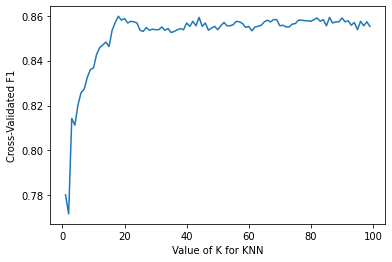
\includegraphics[width=\columnwidth]{knn.pdf}}
\caption{Accuracy vs K before running data reduction}
\label{icml-historical}
\end{center}
\vskip -0.2in
\end{figure}
\subsection{Hyper-parameter Tuning for k in kNN}
We test 100 values of k ranging from 1 to 100 by using 10-fold cross-validation with each k and calculate the cross-validation score for each respective value, this way we are able to determine the best possible value of k along with the accuracy of the classifier.
We examine the best F1 Score for the model and then compare it with the hyper-parameter value to maximize the gradient and find an efficient value.

\subsection{Reducing the Complexity}
To reduce the complexity of the algorithm, we reduce the dimensionality of the data by dropping the misclassified samples and checking the number of good samples to look out for. The whole process is carried out in two steps, first one being data reduction by dropping the misclassified samples, where after splitting our data, we make a prediction with every iteration and identify the misclassified sample and dropping it from the dataset, followed by checking the number of good samples by making a new set of features and values in the new dataset and fitting it into the model to find out the accuracy. You can observe (See figure 2) there is a slight improvement in the overall behavior of noise affecting the dataset resulting in a much smoother curve than before.
\begin{figure}[ht]
\vskip 0.1in
\begin{center}
\centerline{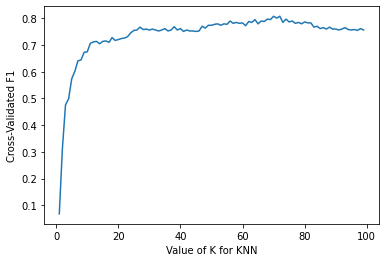
\includegraphics[width=\columnwidth]{knn2.pdf}}
\caption{Accuracy vs K after data reduction}
\label{icml-historical}
\end{center}
\vskip -0.2in
\end{figure}

\subsection{Speeding up the Calculation}

We have learned three algorithms to achieve our goal of speeding up the algorithm. i.e. KDTree, BallTree and Brute Force.

To find out which method is the fastest, we have millis functions both before and after the training and testing commands, which are then compared at the end in seconds.
A trend is observed when we plot all the results (See Figure 3) That both during training and testing time. KDTree proves to be the fastest and Brute Force, the slowest (comparatively) even though the results were highly influential given that the data was balanced.
\begin{figure}[ht]
\vskip 0.1in
\begin{center}
\centerline{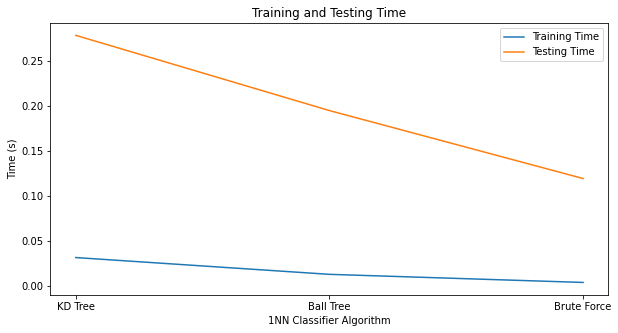
\includegraphics[width=\columnwidth]{knn3.pdf}}
\caption{Comparison of all Three methods for 1NN classifier against Time}
\label{icml-historical}
\end{center}
\vskip -0.2in
\end{figure}


\subsection{Generating Artificial Imbalance}
The last and most crucial experiment to be performed on the test data is generating an artificial imbalance, which we can obtain by simply sampling the data throughout the index of our original dataset and using it to calculate different k in models, then return the average accuracy and f1 score.
We can see that as the value of k increases, our f1 score decreases, making a downward slope (See figure 4). This in turn is not good for the model.

\begin{figure}[ht]
\vskip 0.1in
\begin{center}
\centerline{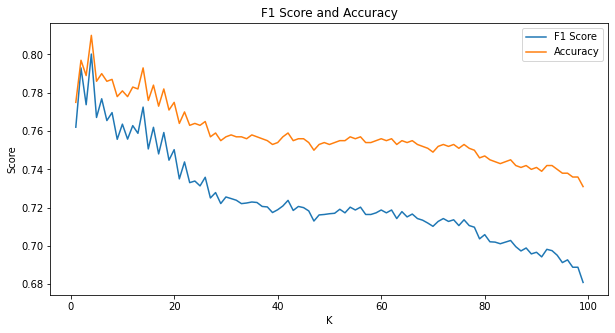
\includegraphics[width=\columnwidth]{knn4.pdf}}
\caption{F1 Score and Accuracy after generating an imbalance
}
\label{icml-historical}
\end{center}
\vskip -0.2in
\end{figure}

\section{Conclusion}
In conclusion, Imbalanced data can cause models to be biased and show unflattering results, as we can see, but any algorithm can be improved by using the techniques mentioned in this project, to obtain a better result. The results above show us that artificially imbalancing the data lead us to have a negative impact on the model accuracy, and the F-Measure proved to be useful as compared to using just accuracy.
If we look at it from an objective set of eyes, if the Bayes Classification provides a better accuracy, we must use all the resources available to compare it to our own methods. 

\end{document}
